\section{Can code language models understand counterfeit samples?} \label{sec:understanding-counterfeit}
In this section, we argue that models struggle to understand counterfeit samples. Due to space limitations, we only highlight a subset of datasets and models in this plot, deferring the complete set of results to Appendix \ref{appendix:all-accuracy-results}. 
\subsection{Correctness Checking}
We begin by examining whether language models can correctly identify whether a program is correct or counterfeit given the natural language specification. In Fig. \ref{fig:execution-accuracy}, we plot the accuracy of CodeLlama 34B, DeepSeek-Coder 33B, GPT-3.5, and GPT-4 on balanced datasets of correct and counterfeit programs for HumanEval and ODEX. For the first three models, the blue bars indicate that correctness checking accuracy is at about 60\% for both of these datasets, which is only slightly better than the 50\% random-guessing baseline. This indicates that models generally fail to distinguish between correct and counterfeit samples. In addition, by comparing the green and red bars, we observe that the performance of these three models on correct samples is much higher than their performance on counterfeit samples, showing that models are biased towards thinking that counterfeit samples are actually correct. On the other hand, GPT-4 is much better (but not perfect) at this task with an accuracy at around 80\% for both datasets. We also observe that in contrast with the rest of the models (including those not shown here, see Fig. \ref{fig:correctness-checking-counterfeit}), GPT-4 is \textit{not} biased towards predicting that these samples are correct. However, GPT-4 still falters around 20\% of the time, and we qualitatively analyze some of these remaining GPT-4 failures in Sec. \ref{sec:qual-analysis}.

\begin{figure}[ht!]
    \centering
    \begin{subfigure}[b]{0.49\columnwidth}
        \centering
        
\includegraphics[width=\textwidth]{figures_v2/main/correctness/correctness_humaneval_codellama-7b.pdf}
        \subcaption{HumanEval (CL-7B)}
    \end{subfigure}
    \hfill
    \begin{subfigure}[b]{0.49\columnwidth}
        \centering
        
\includegraphics[width=\textwidth]{figures_v2/main/correctness/correctness_odex_deepseek-instruct-33b.pdf}
        \subcaption{ODEX (DS-33B)}
    \end{subfigure}
    \caption{Models other than GPT-4 struggle to classify samples as correct or counterfeit and are much better at assessing the correctness of correct samples than counterfeit samples.}
    \label{fig:execution-accuracy}
\end{figure}

\subsection{Execution Prediction}
Next, we assess the ability of models to predict the execution behavior of counterfeit samples. In Fig. \ref{fig:execution-prediction-accuracy}, we plot the execution accuracy of the previous four models on two datasets, LeetCode generated by DS-33B and HumanEval generated by CL-34B. 

In this task, each sample includes a program (correct or counterfeit) $P$ and an input $I$. The accuracy of the correct samples are shown in the green bars. Because counterfeit programs still pass a subset of tests, we distinguish their execution samples into two groups. We call samples where $P$ passes test $I$ \textit{test-passing} counterfeit samples and the rest as \textit{test-failing} counterfeit samples. The execution prediction accuracies of these samples are shown in blue and red, respectively. In purple, we show the proportion of test-failing counterfeit samples where the model actually predicted the output of the correct program. Note that samples counting towards the red accuracy are disjoint from those counting towards the purple accuracy.

Overall, we observe that models have a difficult time distinguishing the semantics of a counterfeit program from their correct counterparts, suggesting they may have a shallow understanding of program semantics. By comparing the green and blue bars with the red bar, we see that models fail much more  at executing counterfeit programs when the semantics are incorrect. The purple bars provide further evidence of this: models other than GPT-4 frequently execute counterfeit programs as if they had the semantics of a correct program, sometimes even more often than their true semantics (red). For GPT-4, the effect is much less pronounced but still present, as GPT-4 still performs much better on correct and test-passing counterfeits than test-failing counterfeits. Despite having such a high performance, it was still confused for a sizable number of test-failing counterfeit samples, predicted the output of the correct program rather than the correct execution result. Overall, as models only see the programs and not the problem statements, this suggests that they may be hallucinating the semantics of incorrect programs. This provides further evidence that models are poor at distinguishing correct programs from counterfeit programs.

\begin{figure}[ht!]
    \centering
    \begin{subfigure}[b]{0.49\columnwidth}
        \centering
        
\includegraphics[width=\textwidth]{figures_v2/main/execution/execution_livecodebench_deepseek-instruct-33b.pdf}
        \subcaption{LeetCode (DS-33B)}
    \end{subfigure}
    \hfill
    \begin{subfigure}[b]{0.49\columnwidth}
        \centering
        
\includegraphics[width=\textwidth]{figures_v2/main/execution/execution_humaneval_codellama-34b.pdf}
        \subcaption{HumanEval (CL-34B)}
    \end{subfigure}
    \caption{Models are much better at executing correct samples than counterfeit samples, and even often execute counterfeit samples as if they were correct.}
    \label{fig:execution-prediction-accuracy}
\end{figure}

\subsection{Repair}
\label{sec:repair}
Finally, we probe the model's ability to repair the counterfeit samples it has generated.
Although this task may appear to simply boil down to code generation,
prior work has highlighted that code understanding forms an integral part of the repair pipeline since achieving good performance hinges on the
model's (in)ability to generate accurate textual explanations of \emph{what} is wrong with the code \cite{olausson2024repair}; as such, self-repair may give us further insight into the model's capabilities.

Prior work has shown that when given information about \emph{which} unit test failed, many models are capable of repairing incorrect Python programs at rates that exceed their baseline pass rates \cite{chen2024teaching,olausson2024repair}.
In this section, we press the model even harder by not giving any execution signal whatsoever, instead simply informing it that the program did not pass; thus, successful repair depends entirely on the model's own ability to understand the program and its relationship to the specification.
Importantly, the success rate of repair must be compared to the baseline pass@1 rate,
since a sample can also be ``repaired'' simply by drawing another unconditional sample from the model.
Details of the experimental setting, and the prompt used for this task, are given in Sec.~\ref{sec:task-eval}-\ref{sec:prompts}.

Fig.~\ref{fig:repair-accuracy} shows the results for CodeLlama 34B\footnote{Since repair is a task that depends heavily on the model adhering to instructions such as actually repairing the programs, rather than re-generating them from scratch, we use the instruction-tuned version CodeLlama 34B-Instruct for these experiments.} and DeepSeek 33B when repairing their own programs on HumanEval and LeetCode (respectively). The full set of results are in Appendix~\ref{appendix:repair}.
In these figures, each point is the mean success rate of repair for a particular problem; points above the line $y=x$ (which corresponds to a pass rate equal to that of the simple resampling strategy) thus indicate successful repair, while points below it indicate that the model could not reliably debug and repair the programs.
We note that although repair appears somewhat successful with DeepSeek-33B on HumanEval (Fig.), beating out the baseline for 35/81 problems, in all other settings a strong majority of the points lie below the line $y=x$. In other words, the success rate of repair is---for most tasks---significantly below what one would achieve with the simple resampling strategy.
This evidence shows that models cannot reliably repair counterfeit samples, which suggests that they could not understand why these programs were deemed incorrect.

\begin{figure}[ht!]
    \centering
    \begin{subfigure}[b]{0.49\columnwidth}
        \centering
        
\includegraphics[width=\textwidth]{figures_v2/main/repair/leetcode/ds33-repairs-ds33-base-50-0.6-2048_scored-scatter-with-base.pdf}
        \subcaption{LeetCode (DS-I-33B)}
    \end{subfigure}
    \hfill
    \begin{subfigure}[b]{0.49\columnwidth}
        \centering
        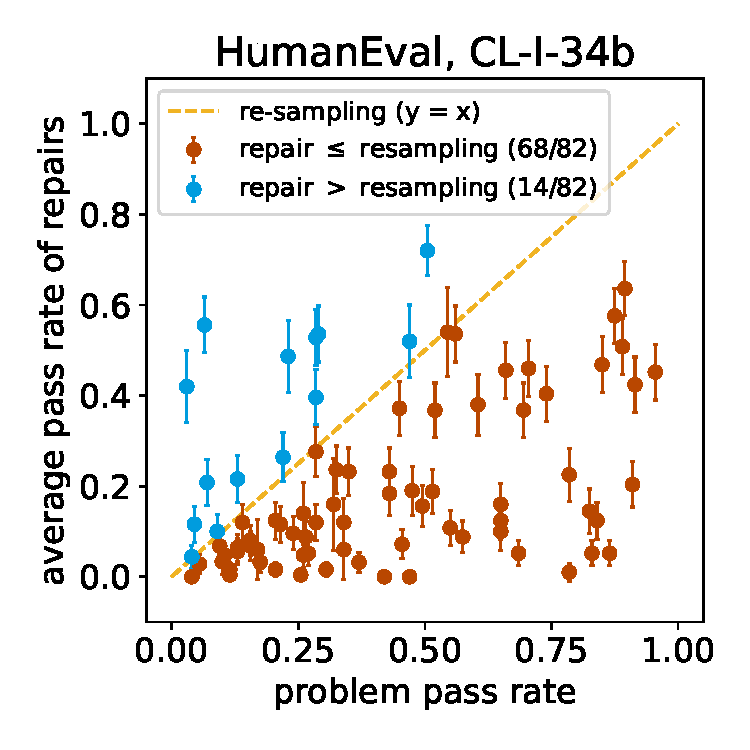
\includegraphics[width=\textwidth]{figures_v2/main/repair/humaneval/filtered_cl34-repairs-cl34-base-50-0.6-2048_scored-scatter-with-base.pdf}
        \subcaption{HumanEval (CL-I-34B)}
    \end{subfigure}
    \caption{In the absence of execution information, we find that repair underperforms resampling in almost all settings. Samples above the $y=x$ resampling baseline have been coloured in blue for clarity. See Appendix~\ref{appendix:repair} for full results. Vertical lines indicate 95\% confidence intervals over repair samples.}
    \label{fig:repair-accuracy}
\end{figure}